\section{Image BERT (iBOT)}
\begin{frame}{}
    \LARGE Contrastive Learning: \textbf{Image BERT Pre-Training with Online Tokenizer (iBOT)}
\end{frame}


\begin{frame}[allowframebreaks]{iBOT}
\begin{figure}
    \centering
    
\includegraphics[width=\linewidth,height=0.9\textheight,keepaspectratio]{images/contrastive/slide_91_2_img.png}
\end{figure}
    \begin{figure}
    \centering
    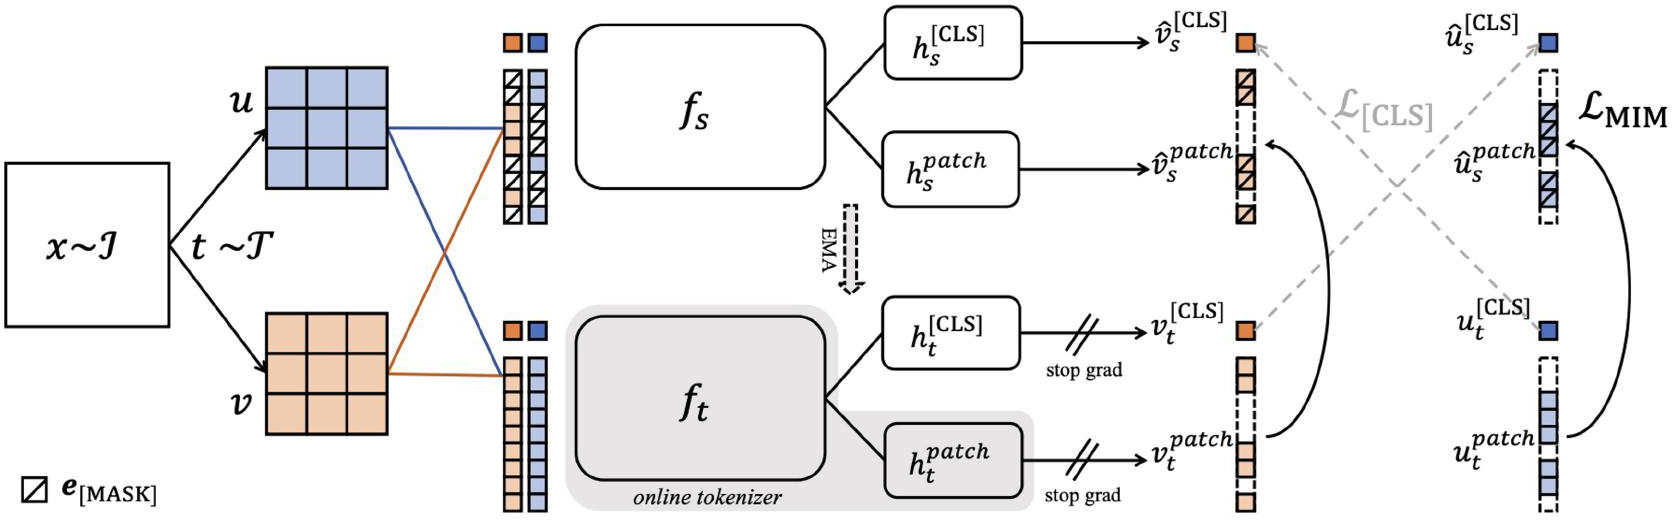
\includegraphics[width=\linewidth,height=0.9\textheight,keepaspectratio]{images/contrastive/slide_91_1_img.png}
\end{figure}

\framebreak

\textbf{Why iBOT?}
\begin{itemize}
    \item Improves self-supervised learning for vision transformers.
    \item Combines two main ideas:
    \begin{itemize}
        \item Learning from missing pieces of images (like solving a puzzle).
        \item Learning by copying a smart teacher model.
    \end{itemize}
\end{itemize}

\framebreak

\textbf{How does it work?}
\begin{itemize}
    \item \textbf{Masked Image Modeling (MIM):} Randomly hide some image patches, so the model has to guess what's missing.
    \item \textbf{Online Distillation:} There's a student model and a teacher model. The student tries to predict both the overall image and the hidden patches, using hints from the teacher.
    \item \textbf{Teacher as EMA:} The teacher isn't trained directly. Instead, it's a slow-moving average of the student, just like in DINO or BYOL.
    \item \textbf{Losses:}
    \begin{itemize}
        \item \textbf{Image-level distillation:} The student learns to match the teacher's understanding of the whole image.
        \item \textbf{Token-level distillation:} The student also learns to match the teacher's guesses for the hidden patches.
    \end{itemize}
\end{itemize}

\framebreak

\begin{columns}[b]
    \column{0.4\textwidth}
        \begin{figure}
            \centering
            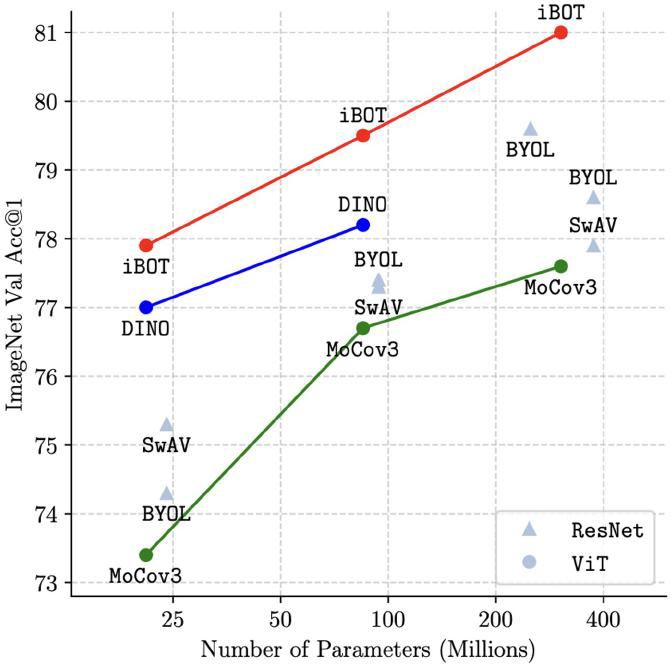
\includegraphics[width=\linewidth,height=0.9\textheight,keepaspectratio]{images/contrastive/slide_92_2_img.png}
        \end{figure}
    \column{0.7\textwidth}
        \begin{figure}
            \centering
            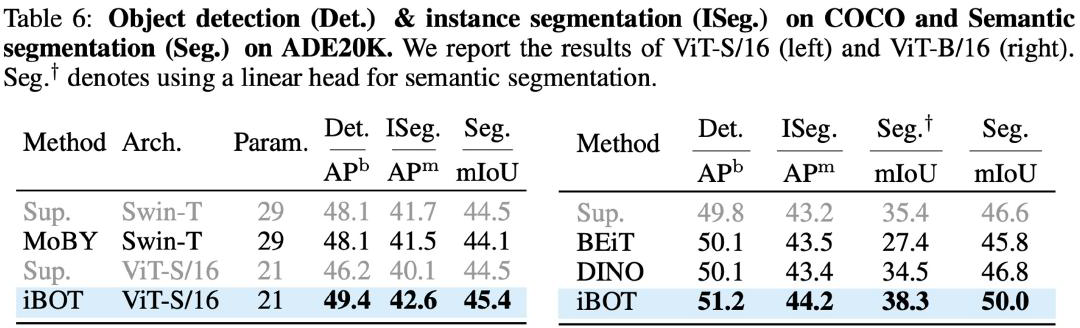
\includegraphics[width=\linewidth,height=0.9\textheight,keepaspectratio]{images/contrastive/slide_92_1_img.png}
        \end{figure}
\end{columns}

\framebreak

\textbf{Why is this cool?}
\begin{itemize}
    \item Mixing MIM and distillation helps the model learn both big-picture (global) and detailed (local) features.
    \item The model can do zero-shot classification—meaning it can recognize new things without extra training—by using prompts, just like CLIP!
\end{itemize}
\end{frame}